
% Copyright 2020 by Robert Hildebrand
%This work is licensed under a
%Creative Commons Attribution-ShareAlike 4.0 International License (CC BY-SA 4.0)
%See http://creativecommons.org/licenses/by-sa/4.0/

%\documentclass[../open-optimization/open-optimization.tex]{subfiles}
%
%\begin{document}
\chapter{Non-linear Programming (NLP)}
\begin{center}
\begin{tabular}{|c|c|}
\hline
$
\min_{x \in \R^n} f(x)
$
& 
$\min_{x \in \R^n} f(x)$ \\
&$ f_i(x) \leq 0  \ \ \text{ for } i=1, \dots, m$\\
&\\
Unconstrained Minimization & Constrained Minimization\\
\hline
\end{tabular}
\end{center}

\begin{itemize}
\item \textbf{objective function} $f \colon \R^n \to \R$
\item may \textbf{maximize} $f$ by minimizing the function $g(x) := -f(x)$
\end{itemize}


\begin{definition}{}{Global and local optima}
The vector $x^*$ is a
\begin{itemize}
\item  \emph{global minimizer} if $f(x^*) \leq f(x) \ \text{ for all } x \in \R^n$.
\item  \emph{local minimizer} if $f(x^*) \leq f(x) \ \text{for all } x \text{ satisfying } \| x- x^*\| \leq \epsilon \text{ for some } \epsilon > 0$.
\item \emph{strict local minimizer} if $f(x^*) < f(x) \ \text{for all } x \neq x^* \text{ satisfying } \| x- x^*\| \leq \epsilon \text{ for some } \epsilon > 0$.
\end{itemize}
\end{definition}

\begin{center}
\includegraphicstatic[scale = 1]{local-min}
\end{center}


\begin{theorem}{Attaining a minimum}{}
Let $S$ be a nonempty set that is closed and bounded.  Suppose that $f \colon S \to \R$ is continuous.  Then the problem $\min\{ f(x) : x \in S\}$ attains its minimum.
\end{theorem}


\begin{definition}{Critical Point}{}
A \emph{critical point} is a point $\bar x$ where $\nabla f(\bar x) = 0$.
\end{definition}

\begin{theorem}{}{}
Suppose that $f\colon \R^n \to \R$ is differentiable.  If $\min\{ f(x) : x \in \R^n\}$ has an optimizer $x^*$, then $x^*$ is a critical point of $f$ (i.e., $\nabla f(x^*) = 0$).
\end{theorem}




\section{Convex Sets}

\begin{definition}{Convex Combination}{}
Given two points $x,y$, a \emph{convex combination} is any point $z$ that lies on the line between $x$ and $y$.  Algebraically, a \emph{convex combination} is any point $z$ that can be represented as $z = \lambda x + (	1-\lambda) y $ for some multiplier $\lambda \in [0,1]$.
\end{definition}

\begin{definition}{Convex Set}{}
A set $C$ is convex if it contains all convex combinations of points in $C$.  That is, for any $x,y \in C$, it holds that $ \lambda x + (1-\lambda) y \in C$ for all $\lambda \in [0,1]$.
\end{definition}
\begin{figure}[h]
  \begin{subfigure}[b]{0.45\textwidth}
    \centering
    \resizebox{\linewidth}{!}{
      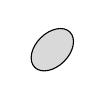
\begin{tikzpicture}[scale = 0.2]
    \draw[rotate=-45,fill=gray!30] (0,0) ellipse (30pt and 45pt);
    %\draw (current bounding box.south east) rectangle (current bounding box.north west);
    \end{tikzpicture}    }
    \caption{Convex Set}
    \label{a}
  \end{subfigure}
  \begin{subfigure}[b]{0.45\textwidth}
    \centering
    \resizebox{\linewidth}{!}{
    
\begin{tikzpicture}[scale = 0.2]
    \useasboundingbox (-1,-1.35) rectangle (1.5,1.35); % values found by trial and error
    \draw[fill=gray!30] (0,0) to [out=140,in=90] (-1,-1)
    to [out=-90,in=240] (0.8,-0.6)
    to [out=60,in=-60] (1.2,1.2)
    to [out=120,in=90] (0.3,0.7)
    to [out=-90,in=20] (0.3,0)
    to [out=200,in=-40] (0,0);
    \draw (-0.5,-0.5) -- (0.7,0.7);
    \fill (-0.5,-0.5) circle[radius=1.5pt];
    \fill (0.7,0.7) circle[radius=1.5pt];
    %\draw (current bounding box.south east) rectangle (current bounding box.north west);
    \end{tikzpicture}
    }
    \caption{Non-convex set}
    \label{b}
  \end{subfigure}
\caption{Examples of convex and non-convex sets.}
\label{fig:convexity}
\end{figure}


\begin{definition}{Convex Sets}{}
A set $S$ is \emph{convex} if for any two points in $S$, the entire line segment between them is also contained in $S$.
That is, for any $x,y \in S$
$$
\lambda x + (1-\lambda y) \in S \ \ \text{ for all } \lambda \in [0,1].
$$
\end{definition}


    


Examples Convex Sets
\begin{enumerate}
    \item \emph{Hyperplane}  $H = \{x \in \R^n : a^\top x = b\}$
    \item \emph{Halfspace}   $H = \{ x \in \R^n : a^\top x \leq b\}$
    \item \emph{Polyhedron}  $P = \{x \in \R^n : Ax \leq b\}$
    \item \emph{Sphere} $S = \{ x \in \R^n : \sum_{i=1}^n x_i^2 \leq 1\}$
    \item \emph{Second Order Cone} $S = \{ (x,t) \in \R^n \times \R : \sum_{i=1}^n x_i^2 \leq t^2 \}$
\end{enumerate}





\begin{definition}{Convex Hull}{}
Let $S\subseteq \R^n$.  The convex hull $\conv(S)$ is the smallest convex set containing $S$.
\end{definition}

\begin{figure}[H]
\begin{center}
\includegraphicstatic[scale = 0.5]{convex-hull-random} \ \ 
\end{center}
\end{figure}
\begin{theorem}{Caratheodory's Theorem}{}
Let $x \in \conv(S)$ and $S \subseteq \R^n$.  Then there exist $x^1, \dots, x^k \in S$ such that $x \in \conv(\{x^1, \dots, x^k\})$ and $k \leq n+1$.
\end{theorem}




\section{Convex Functions}


Convex function are "nice" functions that "open up".  They represent an extremely important class of functions in optimization and typically can be optimized over efficiently.


\begin{figure}[H]
\begin{center}
    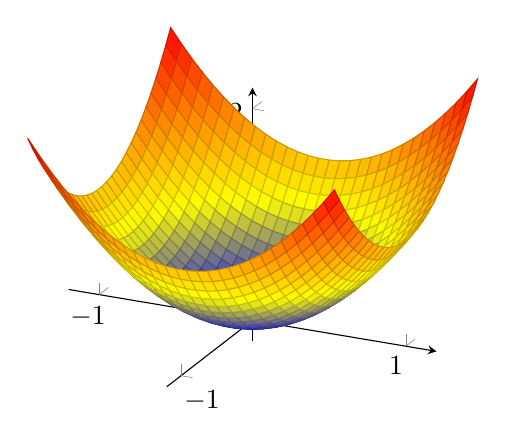
\begin{tikzpicture}[
    declare function = {
        %q(\x) = 5*\x - 1;
        Z(\x,\y) = x^2+y^2; %+ q(\x);
    }]
    \begin{axis}
       [
       axis lines=center,
       enlargelimits,
       tick align=inside,
       domain=-1:1,
       samples=30, 
       %minor tick num=7,
       ]
       \addplot3 [surf] {Z(x,y)};
       %\draw [thick, -latex] (0,0) to [bend right] (0,3);
      % \draw[dashed,line width=0.005\linewidth, ->] (axis cs:-1.1, 1.35, 1) -- (axis cs:0.0,-0.2,0.65);
    \end{axis}
    \end{tikzpicture}
\end{center}
    \caption{Convex Function $f(x,y) = x^2 + y^2$.}
\end{figure} 

\begin{figure}[H]
\begin{center}
    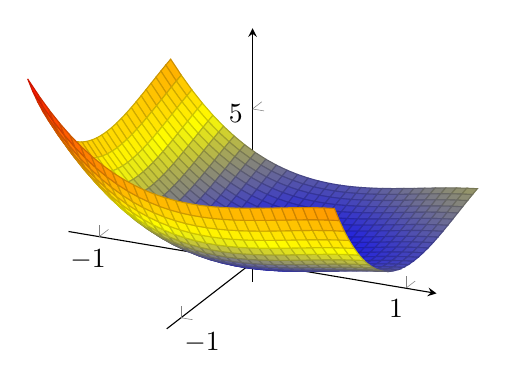
\begin{tikzpicture}[
    declare function = {
        %q(\x) = 5*\x - 1;
        Z(\x,\y) = x^2+y^2- (x - 0.3)^3 - (y - 0.4)^3; %+ q(\x);
    }]
    \begin{axis}
       [
       axis lines=center,
       enlargelimits,
       tick align=inside,
       domain=-1:1,
       samples=30, 
       %minor tick num=7,
       ]
       \addplot3 [surf] {Z(x,y)};
       %\draw [thick, -latex] (0,0) to [bend right] (0,3);
      % \draw[dashed,line width=0.005\linewidth, ->] (axis cs:-1.1, 1.35, 1) -- (axis cs:0.0,-0.2,0.65);
    \end{axis}
    \end{tikzpicture}
\end{center}
    \caption{Non-Convex Function $f(x,y) = x^2 + y^2 - (x - 0.3)^2 - (y - 0.4)^2$.}
\end{figure} 



\begin{definition}{Convex Functions}{}
A function $f \colon \R^n \to \R$ is \emph{convex} if for all $x,y \in \R^n$ and $\lambda \in [0,1]$ we have 
\begin{equation}
\lambda f(x) + (1-\lambda)f(y) \geq f(\lambda x + (1-\lambda) y).
\end{equation}
\end{definition}


\includefiguresource[Illustration explaining the definition of a convex function.][scale = 1]{tikz/convexity-definition.pdf}

\begin{figure}[H]


\end{figure}
\footnotetext{\url{https://tex.stackexchange.com/questions/394923/how-one-can-draw-a-convex-function}}



An equivalent definition of convex function are through the epigraph.

\begin{definition}{Epigraph}{}
The \emph{epigraph} of $f$ is the set $\{(x,y) : y \geq f(x)\}$.  This is the set of all points "above" the function.
\end{definition}

\begin{theorem}{}{}
$f(x)$ is a convex function if and only if the epigraph of $f$ is a convex set.
\end{theorem}

\includegraphicstatic[scale = 0.7]{epigraph.pdf}\footnotemark

\footnotetext{\url{https://tex.stackexchange.com/questions/261501/function-epigraph-possibly-using-fillbetween}}



\begin{example}{Examples of Convex functions}{}

Some examples are 

\begin{itemize}
\item $f(x) = ax + b$
\item $f(x) = x^2$
\item $f(x) = x^4$
\item $f(x) = |x|$
\item $f(x) = e^x$
\item $f(x) = - \sqrt{x}$ on the domain $[0,\infty)$.
\item $f(x) = x^3$ on the domain $[0,\infty)$.
\item $f(x,y) = 
\sqrt{x^2 + y^2}$
\item $f(x,y) = x^2 + y^2 + x$
\item $ f(x,y) = e^{x+y}$
\item $f(x,y) = e^{x} + e^{y} + x^2+  (3x + 4y)^6$
\end{itemize}

\end{example}






\begin{figure}[H]
\begin{center}
    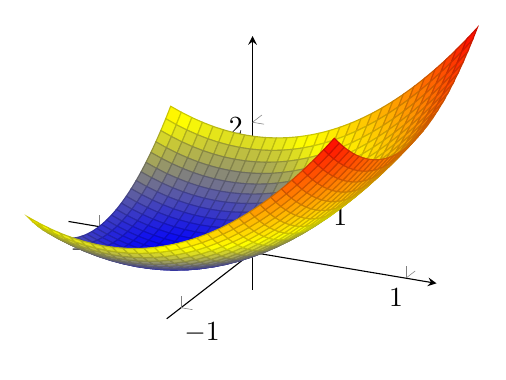
\begin{tikzpicture}[
    declare function = {
        %q(\x) = 5*\x - 1;
        Z(\x,\y) = x^2+y^2 + x; %+ q(\x);
    }]
    \begin{axis}
       [
       axis lines=center,
       enlargelimits,
       tick align=inside,
       domain=-1:1,
       samples=30, 
       %minor tick num=7,
       ]
       \addplot3 [surf] {Z(x,y)};
       %\draw [thick, -latex] (0,0) to [bend right] (0,3);
      % \draw[dashed,line width=0.005\linewidth, ->] (axis cs:-1.1, 1.35, 1) -- (axis cs:0.0,-0.2,0.65);
    \end{axis}
    \end{tikzpicture}
     \hspace{1cm}
    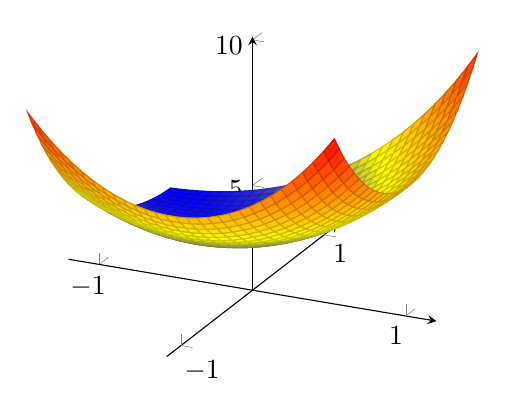
\begin{tikzpicture}[
    declare function = {
        %q(\x) = 5*\x - 1;
        Z(\x,\y) = exp(x+y) + exp(x-y) + exp(-x-y); %+ q(\x);
    }]
    \begin{axis}
       [
       axis lines=center,
       enlargelimits,
       tick align=inside,
       domain=-1:1,
       samples=30, 
       %minor tick num=7,
       ]
       \addplot3 [surf] {Z(x,y)};
       %\draw [thick, -latex] (0,0) to [bend right] (0,3);
      % \draw[dashed,line width=0.005\linewidth, ->] (axis cs:-1.1, 1.35, 1) -- (axis cs:0.0,-0.2,0.65);
    \end{axis}
    \end{tikzpicture}
    \hspace{1cm}
     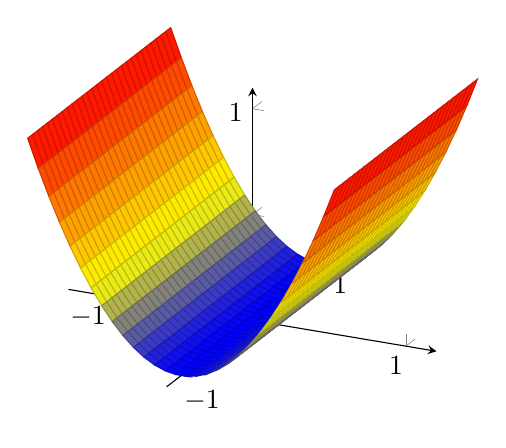
\begin{tikzpicture}[
    declare function = {
        %q(\x) = 5*\x - 1;
        Z(\x,\y) = x^2; %+ q(\x);
    }]
    \begin{axis}
       [
       axis lines=center,
       enlargelimits,
       tick align=inside,
       domain=-1:1,
       samples=30, 
       %minor tick num=7,
       ]
       \addplot3 [surf] {Z(x,y)};
       %\draw [thick, -latex] (0,0) to [bend right] (0,3);
      % \draw[dashed,line width=0.005\linewidth, ->] (axis cs:-1.1, 1.35, 1) -- (axis cs:0.0,-0.2,0.65);
    \end{axis}
    \end{tikzpicture}
\end{center}
    \caption{Convex Functions $f(x,y) = x^2 + y^2+ x$ ,  $f(x,y) = e^{x+y} + e^{x-y} + e^{-x-y} $, and $f(x,y) = x^2 $.}
\end{figure} 





\subsection{Proving Convexity - Characterizations}

\begin{theorem}{Convexity: First order characterization - linear underestimates}{}{}
Suppose that $f\colon \R^n \to \R$ is differentiable.  Then $f$ is convex if and only if for all $\bar x \in \R^n$, then linear tangent is an underestimator to the function, that is,
$$
f(\bar x) + (x - \bar x)^\top \nabla f(\bar x) \leq f(x).
$$
\end{theorem}

\begin{figure}[H]
\begin{center}
\includegraphicstatic[scale = 0.12, trim = {0 0 0 10cm}, clip ]{first-order-convexity}\footnotemark
\end{center}
\end{figure}
\footnotetext{\url{https://machinelearningcoban.com/2017/03/12/convexity/}}



\begin{theorem}{Convexity: Second order characterization - positive curvature}{}
We give statements for uni-variate functions and multi-variate functions.
\begin{itemize}
\item Suppose $f \colon \R \to \R$ is twice differentiable.  Then $f$ is convex if and only if $f''(x) \geq 0$ for all $x \in \R$.
\item Suppose $f \colon \R^n \to \R$ is twice differentiable.  Then $f$ is convex if and only if $\nabla^2 f(x) \succcurlyeq 0$ for all $x \in \R^n$.
\end{itemize}
\end{theorem}


\subsection{Proving Convexity - Composition Tricks}


\begin{general}{Positive Scaling of Convex Function is Convex}{}
If $f$ is convex and $\alpha > 0$, then $\alpha f$ is convex. 

\textcolor{blue}{\textbf{Example: } $f(x) = e^x$ is convex.  Therefore, $25 e^x$ is also convex.}
\end{general}

\begin{general}{Sum of Convex Functions is Convex}{}
If $f$ and $g$ are both convex, then $f+g$ is also convex.

\textcolor{blue}{\textbf{Example: } $f(x) = e^x, g(x) = x^4$ are convex.  Therefore, $e^x + x^4$ is also convex.}
\end{general}

\begin{general}{Composition with affine function}{}
If $f(x)$ is convex, then $f(a^\top x + b)$ is also convex.

\textcolor{blue}{\textbf{Example: } $f(x) = x^4$ are convex.  Therefore, $(3x + 5y + 10z)^4$ is also convex.}
\end{general}

\begin{general}{Pointwise maximum}{}
If $f_i$ are convex for $i=1, \dots, t$, then $f(x) = \max_{i=1, \dots, t} f_i(x)$ is convex.

\textcolor{blue}{\textbf{Example: } $f_1(x) = e^{-x}$, $f_2(x) = e^{x}$ are convex.  Therefore, $f(x) = \max(e^x, e^{-x})$ is also convex.}
\end{general}

\begin{general}{Other compositions}{}
Suppose 
$$
f(x) = h(g(x)).
$$
\begin{enumerate}
\item If $g$ is convex, $h$ is convex and \textbf{non-decreasing}, then $f$ is convex.
\item If $g$ is concave, $h$ is convex and \textbf{non-increasing}, then $f$ is convex.
\end{enumerate}

\textcolor{blue}{\textbf{Example 1: } $g(x) = x^4$ is convex, $h(x) = e^{x}$ is convex and non-decreasing.  Therefore, $f(x) = e^{x^4}$ is also convex.}\\

\textcolor{blue}{\textbf{Example 2: } $g(x) = \sqrt{x}$ is concave (on $[0,\infty)$), $h(x) = e^{-x}$ is convex and non-increasing.  Therefore, $f(x) = e^{-\sqrt{x}}$ is convex on $x \in [0,\infty)$.}
\end{general}







\section{Convex Optimization Examples}
\subsection{Unconstrained Optimization: Linear Regression}

Given data points $x^1, \dots, x^N \in \R^d$ and out values $y^i \in \R$, we want to find a linear function $y = \beta \cdot x$ that best approximates $x^i \cdot \beta \approx y^i$.  For example, the data could $x = (\text{time})$ and the output could be $y = \text{position}$.  


\includefiguresource[Line derived through linear regression.][scale = 1]{tikz/linear-regression.pdf}

\begin{figure}[H]
\begin{center}



\includegraphicstatic[scale = 1]{LinearRegression.pdf}\footnotemark
\end{center}
\end{figure}
\footnotetext{\url{https://latexdraw.com/linear-regression-in-latex-using-tikz/}}



As is standard, we choose the error (or "loss") from each data point as the squared error.  Hence, we can model this as the optimization problem:
\begin{align}
\label{eq:least-squares}
\min_{\beta \in \R^d} & \sum_{i=1}^N (x^i \cdot \beta - y^i)^2
\end{align}

This problem has a nice closed form solution.  We will derive this solution, and then in a later section discuss why using this solution might be too  slow to compute on large data sets.  In particular, the solution comes as a system of linear equations.  But when $N$ is really large, we may not have time to solve this system, so an alternative is to use decent methods, discussed later in this chapter.

\begin{theorem}{Linear Regression Solution}{}
The solution to \eqref{eq:least-squares} is 
\begin{equation}
\beta = (X^\top X)^{-1} X^\top Y,
\end{equation}
where 
$$X = 
\begin{bmatrix}
x^1\\
\vdots \\
x^N
\end{bmatrix}
= 
\begin{bmatrix}
x^1_1 & x^1_2 & \dots & x^1_d\\
\vdots \\
x^N_1 & x^N_2 & \dots & x^N_d
\end{bmatrix}
$$
\end{theorem}
\begin{proof}
Solve for $\nabla f(\beta) = 0$.

To be completed....
\end{proof}

\begin{resource}
\url{https://www.youtube.com/watch?v=E5RjzSK0fvY}
\end{resource}



\section{Machine Learning - SVM}



%\includegraphics[scale = 0.2]{scikitlearn}
\emph{Support Vector Machine} (SVM) is a tool used in machine learning for classifying data points.   For instance, if there are red and black data points, how can we find a good line that separates them?  The input data that you are given is as follows:

\paragraph{Input:}
\begin{itemize}
\item $d$-dimensional data points $x^1, \dots, x^N$ 
\item $1$-dimensional labels $z^1, \dots, z^N$  (typically we will use $z_i$ is either $1$  or $-1$)
\end{itemize}

The output to the problem should he a hyperplane $w^\top x + b = 0$ that separates the two data types (either exact separation or approximate separation).

\paragraph{Output:}
\begin{itemize}
\item A $d$-dimensional vector $w$
\item A $1$-dimensional value $b$
\end{itemize}

Given this output, we can construct a classification function $f(x)$ as 

\begin{equation}
f(x) = \begin{cases}
1 & \text{ if } w^\top x + b \geq 0,\\
-1 & \text{ if } w^\top x + b < 0.
\end{cases}
\end{equation}




There are three versions to consider:

\subsubsection{Feasible separation}

If we only want to a line that separates the data points, we can use the following optimization model.

\begin{align*}
\min \quad & 0 \\
\text{ such that } \quad & z^i( w^\top x^i + b) \geq 1 & \text{ for all } i=1, \dots, N\\
& w  \in \R^d\\
& b \in \R
\end{align*}
\subsubsection{Distance between hyperplanes}

We want to know a formula for the distance between two parallel hyperplanes.   In particular, we will look at the hyperplane $H_0 = \{ x :  h^\top x = 0\}$ and $H_1 = \{x : h^\top x = 1\}$.

We choose a point $x^0 = 0 \in H_0$, and then find the point in $H_1$ that minimizes the distance between these two points.

This can be phrased as the optimization problem

\begin{align*}
\min &  \|x \|_2\\
 \text{ s.t. } & h^\top x = 1
\end{align*}

For convenience, we will solve this problem instead:
\begin{align*}
\min &  \|x \|_2^2\\
 \text{ s.t. } & h^\top x = 1
\end{align*}

We will rewrite this problem by removing the equation.   We assume, without loss of genearlity, that $h_n \neq 0$.  Otherwise, reorder the variables.

So, since $h_n \neq 0$, we have 
$$
1 = h_1 x_1 + \dots + h_n x_n
$$
and hence
$$
x_n = \frac{1 - h_1 x_1 + \dots + h_{n-1}x_{n-1}}{h_n}.
$$

Now we can re-write the optimzation problem as the unconstrainted optimization problem 

\begin{align*}
\min &  f(x) := x_1^2 + \dots + x_{n-1}^2 + \left( \frac{1 - h_1 x_1 + \dots + h_{n-1}x_{n-1}}{h_n}\right)^2\\
\end{align*}

First, note that $f(x)$ is a strictly convex function.   Thus, we can find the optimal solution by computing where the gradient vanishes.

$$
\nabla f(x) = \begin{bmatrix}
\vdots \\
2x_i + 2\frac{h_i}{h_n}\left( \frac{1 - h_1 x_1 + \dots + h_{n-1}x_{n-1}}{h_n}\right)\\
\vdots
\end{bmatrix} = 0
$$
But notice what happens when we substitue back in $x_n$.  We obtain
$$
\nabla f(x) = \begin{bmatrix}
\vdots \\
2x_i + 2\frac{h_i}{h_n}x_n\\
\vdots
\end{bmatrix} = 0
$$
Taking the $i$th equation, we have

$$
\frac{x_i}{h_i} = \frac{x_n}{h_n} \ \ \text{ for all } i=1, \dots, n-1.
$$

Let $\lambda = \frac{x_n}{h_n}$.  Then for all $i=1, \dots, n$, we have $x_i = \lambda h_i$, or in vector form, we have
$$
x = \lambda h.
$$

Thus, we can go back the original optimization problem and look only at solutions that are of the form $x = \lambda h$.

Plugging this into the original model, we have

\begin{align*}
\min &  \|\lambda h \|_2 \\
 \text{ s.t. } & h^\top (\lambda h)= 1
\end{align*}
which is equivalent to
\begin{align*}
\min &   \lambda \|h\|_2\\
 \text{ s.t. } & \lambda = \frac{1}{h^\top  h}.
\end{align*}

Recall that $h^\top h = \|h\|_2^2$.

Thus, the minimum distance is exactly 

$$
\frac{1}{\|h\|_2^2} \|h\|_2 = \frac{1}{\|h\|_2}
$$

\subsubsection{SVM}
We can modify the objective function to find a best separation between the points.  This can be done in the following way


\begin{center}
\includegraphicstatic[scale = 0.75]{svm2}
\end{center}



\begin{align*}
\min \quad & \|w\|_2^2 \\
\text{ such that } \quad & z^i( w^\top x^i + b) \geq 1 & \text{ for all } i=1, \dots, N\\
& w  \in \R^d\\
& b \in \R
\end{align*}

Here, $\|w\|_2^2 = \sum_{i=1}^d w_i^2 = w_1^2 + \dots + w_d^2$.


\subsubsection{Approximate SVM}
We can modify the objective function and the constraints to allow for approximate separation.  This would be the case when you want to ignore outliers that don't fit well with the data set, or when exact SVM is not possible.  This is done by changing the constraints to be 
$$
z^i( w^\top x^i + b) \geq 1 - \delta_i
$$
where $\delta_i\geq 0$ is the error in the constraint for datapoint $i$.  In order to reduce these errors, we add a penalty term in the objective function that encourages these errors to be small.  For this, we can pick some number $C$ and write the objective as 
$$
\min  \|w\|_2^2  + C \sum_{i=1}^N \delta_i.
$$

This creates the following optimization problem
\begin{align*}
\min \quad & \|w\|_2^2+ C \sum_{i=1}^N \delta_i \\
\text{ such that } \quad & z^i( w^\top x^i + b) \geq 1  - \delta_i& \text{ for all } i=1, \dots, N\\
& w  \in \R^d\\
& b \in \R\\
& \delta_i \geq 0  \text { for all } i =1, \dots, N
\end{align*}


See information about the scikit-learn module for svm here:
\url{https://scikit-learn.org/stable/modules/svm.html}.

\subsection{SVM with non-linear separators}



\begin{resource}
\url{https://www.youtube.com/watch?time_continue=6&v=N1vOgolbjSc}
\end{resource}



Suppose for instance you are given data $x^1, \dots, x^N \in \R^2$ (2-dimensional data) and given labels are dependent on the distance from the origin, that is,  all data points $x$ with  $x_1^2 + x_2^2 > r$ are given a label $+1$ and all data points with $x_1^2 + x_2^2 \leq r$ are given a label $-1$.   That is, we want to learn the function 

\begin{equation}
f(x) = \begin{cases}
1 & \text{ if } x_1^2 + x_2^2 >  r,\\
-1 & \text{ if } x_1^2 + x_2^2 \leq r.
\end{cases}
\end{equation}

\begin{example}{}{}
\begin{center}
\includegraphicstatic[scale = 0.3]{svm-nonlinear} \ \ \includegraphicstatic[scale = 0.3]{svm-nonlinear-training}
\end{center}
Here we have a classification problem where the data cannot be separated by a hyperplane.  On the left, we have all of the data given to use.  On the right, we have a subset of the data that we could try using for training and then test our learned function on the remaining data.  As we saw in class, this amount of data was not sufficient to properly classify most of the data.
\end{example}

We cannot learn this classifier from the data directly using the hyperplane separation with SVM in the last section.  But, if we modify the data set, then we can do this.  

For each data point $x$, we transform it into a data point $X$ by adding a third coordinate equal to $x_1^2 + x_2^2$.  That is 
\begin{equation}
x = \begin{pmatrix} x_1 \\ x_2 \end{pmatrix} \quad \rightarrow \quad X = \begin{pmatrix} x_1 \\ x_2 \\ x_1^2 + x_2^2 \end{pmatrix}.
\end{equation}
In this way, we convert the data $x^1, \dots, x^N$ into data $X^1, \dots, X^N$ that lives in a higher-dimensional space.  But with this new dataset, we can apply the hyperplane separation technique in the last section to properly classify the data.

This can be done with other nonlinear classification functions.  

\subsection{Support Vector Machines}

\begin{general}{Support Vector Machine - Exact Classification}{}
Given labeled data $(x^i, y_i)$ for $i=1, \dots, N$, where $x^i \in \R^d$ and $y^i \in \{-1,1\}$, find a vector $w \in \R^d$ and a number $b \in \R$ such that 
\begin{align}
x^i \cdot w + b & > 0  & \text{ if } y^i = 1\\
x^i \cdot w + b & < 0  & \text{ if } y^i = -1
\end{align}
\end{general}

There may exist many solutions to this problem.  Thus, we are interested in the "best" solution.  Such a solution will maximize the separation between the two sets of points.  To consider an equal margin on either size, we set the right hand sides to 1 and -1 and then compute the margin form the hyperplane.  Notice that it is sufficient to use 1 and -1 on the right hand sides since any scaling can happen in $w$ and $b$.

\begin{center}
\includegraphicstatic[scale = 0.75]{svm2}
\end{center}
We will show that the margin under this model can be computed as $\frac{2}{\|w\|}$ where $\|w\| = \sqrt{w_1^2 +  \dots + w_d^2}$.  Hence,  maximizing the margin is equivalent to minimizing $w_1^2 +  \dots + w_d^2$.  We arrive at the model

\begin{align}
\min & \sum_{i=1}^d w_i^2\\
&x^i \cdot w + b  \geq 1  & \text{ if } y^i = 1\\
&x^i \cdot w + b  \leq -1  & \text{ if } y^i = -1
\end{align}

Or even more compactly written as 
\begin{align}
\min & \sum_{i=1}^d w_i^2\\
&y^i(x^i \cdot w + b) \geq 1  & \text{ for } i=1, \dots, N
\end{align}






\section{Classification}



\subsection{Machine Learning}

\begin{resource}
\url{https://www.youtube.com/watch?v=bwZ3Qiuj3i8&list=PL9ooVrP1hQOHUfd-g8GUpKI3hHOwM_9Dn&index=13}


\url{https://towardsdatascience.com/solving-a-simple-classification-problem-with-python-fruits-lovers-edition-d20ab6b071d2}
\end{resource}
\subsection{Neural Networks}

\begin{resource}
\url{https://www.youtube.com/watch?v=bVQUSndDllU}

\url{https://www.youtube.com/watch?v=8bNIkfRJZpo}

\url{https://www.youtube.com/watch?v=Dws9Zveu9ug}
\end{resource}


\section{Box Volume Optimization in Scipy.Minimize}
\url{https://www.youtube.com/watch?v=iSnTtV6b0Gw}

\section{Modeling}
We will discuss a few models and mention important changes to the models that will make them solvable.  

\paragraph{Important tips}
\begin{enumerate}
\item \textbf{Find a convex formulation.}  It may be that the most obvious model for your problem is actually non-convex.  Try to reformulate your model into one that is convex and hence easier for solvers to handle.
\item \textbf{Intelligent formulation.}  Understanding the problem structure may help reduce the complexity of the problem.  Try to deduce something about the solution to the problem that might make the problem easier to solve.  This may work for special cases of the problem.
\item \textbf{Identify problem type and select solver.}  Based on your formulation, identify which type of problem it is and which solver is best to use for that type of problem.  For instance, \gurobi can handle some convex quadratic problems, but not all.  \ipopt is a more general solver, but may be slower due to the types of algorithms that it uses.

\item \textbf{Add bounds on the variables.} Many solvers perform much better if they are provided bounds to the variables.  This is because it reduces the search region where the variables live.   Adding good bounds could be the difference in the solver finding an optimal solution and not finding any solution at all.
\item \textbf{Warm start.} If you know good possible solutions to the problem (or even just a feasible solution), you can help the solver by telling it this solution.  This will reduce the amount of work the solver needs to do.  In \jump this can be done by using the command \textit{setvalue(x,[2 4 6])}, where here it sets the value of vector $x$ to $[2\ 4\ 6]$.  It may be necessary to specify values for all variables in the problem for it to start at.
\item \textbf{Rescaling variables.} It sometimes is useful to have all variables on the same rough scale.  For instance, if minimizing $x^2 + 100^2 y^2$, it may be useful to define a new variable $\bar y = 100y$ and instead minimize $x^2 + \bar y^2$.
\item \textbf{Provide derivatives.} Working out gradient and hessian information by hand can save the solver time.  Particularly when these are sparse (many zeros).  These can often be provided directly to the solver.
\end{enumerate}
See \url{http://citeseerx.ist.psu.edu/viewdoc/download;jsessionid=4982C26EC5F25564BCC239FD3785E2D3?doi=10.1.1.210.3547&rep=rep1&type=pdf} for many other helpful tips on using \ipopt.
\subsection{Minimum distance to circles}

The problem we will consider here is:
Given $n$ circles, find a center point that minimizes the sum of the distances to all of the circles. 

\begin{general}{Minimize distance to circles}{}%\polynomial}
Given circles described by center points $(a_i, b_i)$ and radius $r_i$ for $i=1, \dots, n$, find a point $c = (c_x,c_y)$ that minimizes the sum of the distances to the circles.  \\
\end{general}

\begin{center}
\includegraphicstatic[scale = 0.3]{circles-figure}
\end{center}

\begin{general}{Minimize distance to circles - Model attempt $\#1$}{Non-convex}
Let $(x_i,y_i)$ be a point in circle $i$.  Let $w_i$ be the distance from $(x_i, y_i)$ to $c$.  Then we can  model the problem as follows:
\begin{equation}
\begin{array}{rlr}
\min \quad & \sum_{i=1}^3 w_i \hfill & \text{ Sum of distances}\\
\text{ s.t. } &  \sqrt{(x_i - a_i)^2  + (y_i - b_i)^2}  = r , \ \ i=1,\dots, n& \text{ $(x_i, y_i)$ is in circle $i$}\\
& \sqrt{(x_i - c_x)^2 + (y_i - c_y)^2} = w_i \ \ i=1, \dots, n & \text{$w_i$ is distance from $(x_i, y_i)$ to $c$}\\
\end{array}
\end{equation}
\end{general}

\textbf{This model has several issues:}
\begin{enumerate}
\item  If the center $c$ lies inside one of the circles, then the constraint  $\sqrt{(x_i - a_i)^2  + (y_i - b_i)^2}  = r$ may not be valid.  This is because the optimal choice for $(x_i,y_i)$ in this case would be inside the circle, that is, satisfying $ \sqrt{(x_i - a_i)^2  + (y_i - b_i)^2}  \leq r$.
\item This model is \textbf{nonconvex}.  In particular the equality constraints make the problem nonconvex.
\end{enumerate}

Fortunately, we can relax the problem to make it convex an still model the correct solution.  In particular, consider the constraint 
$$
 \sqrt{(x_i - c_x)^2 + (y_i - c_y)^2} = w_i .
$$
Since we are minimizing $\sum w_i$, it is equivalent to have the constraint
$$
 \sqrt{(x_i - c_x)^2 + (y_i - c_y)^2} \leq w_i.
$$
This is equivalent because any optimal solution make $w_i$ the smallest it can, and hence will meet that constraint at equality.  

What is great about this change, it that it makes the constraint \textbf{convex!}. To see this we can write $f(z) = \|z\|_2^2$, $z = (x_i - c_x, y_i - x_y)$.  Since $f(z)$ is convex and the transformation into variables $x_i, c_x, y_i, c_y$ is linear, we have that $f(x_i - c_x, y_i - x_y)$ is convex.   Then since $-w_i$ is linear, we have that
$$
f(x_i - c_x, y_i - x_y) - w_i
$$
is a convex function.  Thus, the constraint 
$$
f(x_i - c_x, y_i - x_y) - w_i \leq 0 
$$
is a convex constraint.


This brings us to our second model.


\begin{general}{Minimize distance to circles - Model attempt $\#2$}{Convex}
Let $(x_i,y_i)$ be a point in circle $i$.  Let $w_i$ be the distance from $(x_i, y_i)$ to $c$.  Then we can  model the problem as follows:
\begin{equation}
\begin{array}{rlr}
\min \quad & \sum_{i=1}^3 w_i \hfill & \text{ Sum of distances}\\
\text{ s.t. } &  \sqrt{(x_i - a_i)^2  + (y_i - b_i)^2}  \leq r , \ \ i=1,\dots, n& \text{ $(x_i, y_i)$ is in circle $i$}\\
& \sqrt{(x_i - c_x)^2 + (y_i - c_y)^2}\leq w_i \ \ i=1, \dots, n & \text{$w_i$ is distance from $(x_i, y_i)$ to $c$}\\
\end{array}
\end{equation}
\end{general}

Lastly, we would like to make this model better for a solver.  For this we will

\begin{enumerate}
\item Add bounds on all the variables
\item Change format of non-linear inequalities
\end{enumerate}

\begin{general}{Minimize distance to circles - Model attempt $\#3$}{Convex}
Let $(x_i,y_i)$ be a point in circle $i$.  Let $w_i$ be the distance from $(x_i, y_i)$ to $c$.  Then we can  model the problem as follows:
\begin{equation}
\begin{array}{rlr}
\min \quad & \sum_{i=1}^3 w_i \hfill & \text{ Sum of distances}\\
\text{ s.t. } & (x_i - a_i)^2  + (y_i - b_i)^2  \leq r^2 , \ \ i=1,\dots, n& \text{ $(x_i, y_i)$ is in circle $i$}\\
& (x_i - c_x)^2 + (y_i - c_y)^2\leq w_i^2 \ \ i=1, \dots, n & \text{$w_i$ is distance from $(x_i, y_i)$ to $c$}\\
& 0 \leq w_i \leq u_i\\
& a_i - r \leq x_i \leq a_i + r\\
& b_i -r \leq y_i \leq b_i + r\\
\end{array}
\end{equation}
\end{general}

\begin{examplewithcode}{Minimize distance to circles}{NLP:Circles-Problem}
Here we minimize the distance of three circles of radius 1 centered at $(0,0)$, $(3,2)$, and $(0,5)$.  
Note: The bounds on the variables here are not chosen optimally. 
\begin{align*}\min\quad & w_{1} + w_{2} + w_{3}\\
\text{Subject to} \quad & (x_{1} - 0) ^ 2 + (y_{1} - 0)^ 2  \leq 1\\
 & (x_{2} - 3) ^ 2 + (y_{2} - 2) ^ 2)  \leq 1\\
 & (x_{3} - 0) ^ 2 + (y_{3} - 5) ^ 2)  \leq 1\\
 & (x_{1} - c_x) ^ 2 + (y_{1} - c_y) ^ 2) \leq w_{1}^ 2\\
 & (x_{2} - c_x) ^ 2 + (y_{2} - c_y) ^ 2\leq w_{2}^ 2\\
 & (x_{3} - c_x) ^ 2 + (y_{3} - c_y) ^ 2\leq w_{3}^ 2\\
 & -1 \leq x_{i} \leq 10 \quad\forall i \in \{1,2,3\}\\
 & -1 \leq y_{i} \leq 10 \quad\forall i \in \{1,2,3\}\\
 & 0 \leq w_{i} \leq 40 \quad\forall i \in \{1,2,3\}\\
 & -1 \leq c_x \leq 10\\
 & -1 \leq c_y \leq 10\\
\end{align*}
\end{examplewithcode}


\section{Machine Learning}
There are two main fields of machine learning:
\begin{itemize}
\item Supervised Machine Learning,
\item Unsupervised Machine Learning.
\end{itemize}
Supervised machine learning is composed of \emph{Regression} and \emph{Classification}.  This area is thought of as being given labeled data that you are then trying to understand the trends of this labeled data.

Unsupervised machine learning is where you are given unlabeled data and then need to decide how to label this data. For instance, how can you optimally partition the people in a room into 5 groups that share the most commonalities?

\section{Machine Learning - Supervised Learning - Regression}
See the video lecture information.


\section{Machine learning - Supervised Learning - Classification}
The problem of data \emph{classification} begins with \emph{data} and \emph{labels}.  The goal is \emph{classification} of future data based on sample data that you have by constructing a function to understand future data.
\begin{center}
\textit{
\textbf{Goal:} Classification - create a function $f(x)$ that takes in a data point $x$ and outputs the correct label.}
\end{center}

These functions can take many forms.  In binary classification, the label set is $\{+1, -1\}$, and we want to correctly (as often as we can) determine the correct label for a future data point.

There are many ways to determine such a function $f(x)$.  In the next section, we will learn about SVM that determines the function by computing a hyperplane that separates the data labeled $+1$ from the data labeled $-1$.

Later, we will learn about \emph{neural networks} that describe much more complicated functions.  

Another method is to create a \emph{decision tree}.  These are typically more interpretable functions (neural networks are often a bit mysterious) and thus sometimes preferred in settings where the classification should be easily understood, such as a medical diagnosis.  We will not discuss this method here since it fits less well with the theme of nonlinear programming.




\subsection{Python SGD implementation and video}
\url{https://github.com/llSourcell/Classifying_Data_Using_a_Support_Vector_Machine/blob/master/support_vector_machine_lesson.ipynb}



%
%\end{document}
